%%%%%%%%%%%%%%%%%%%%%%%%%%%%%%%%%%%%%%%%%
% University/School Laboratory Report
% LaTeX Template
% Version 2.0 (4/12/12)
%
% This template has been downloaded from:
% http://www.latextemplates.com
%
% License:
% CC BY-NC-SA 3.0 (http://creativecommons.org/licenses/by-nc-sa/3.0/)
%
% Original header:
%
% This is a LaTeX version of the sample laboratory report
% from Virginia Tech's copyrighted 08-09 CHEM 1045/1046 lab manual.
% Reproduction of this one appendix section for academic purposes
% should fall under fair use.
%
%%%%%%%%%%%%%%%%%%%%%%%%%%%%%%%%%%%%%%%%%

\documentclass{article}
\usepackage{graphicx}
\usepackage{float}
\usepackage{mathtools}

\title{ELEC 302-81\\ Lab 2\\ Transformer Fundamentals} % Title
% \author{John \textsc{Smith}} % Author name
\date{\today} % Specify a date for the report

\begin{document}

\maketitle

\begin{center}
  \begin{tabular}{lr}
    Date Performed: & January 28, 2013 \\
    Partners: & Rawley Dent \\
              & Charles Pittman \\
    Instructor: & Dr. Weatherford
  \end{tabular}
\end{center}

\pagebreak

%\setlength\parindent{0pt} % Removes all indentation from paragraphs

\section{Purpose of Experiment}
CHANGE ME!! In this experiment, an RLC circuit was modeled on an EMS
workstation.  The capacitance was varied for two different inductance values.
The circuit was then analyzed to obtain measured values for the circuit power
factor, real power, and apparent power. These measured results were then
compared to the theoretical values calculated beforehand. Familiarization with
the EMS workstation was also obtained.

\section{Circuits Tested}
\subsection{Voltage Ratios}
\begin{figure}[H]
  \centering
  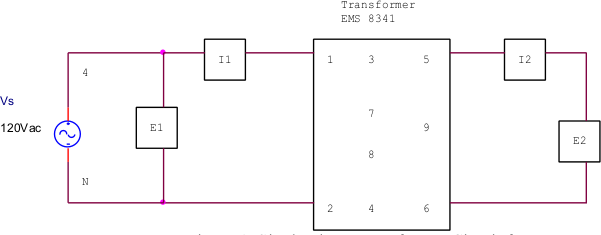
\includegraphics[width=.8\textwidth]{img/circuit_01}
  \caption{Single Phase Transformer Circuit}
  \label{fig:circuit_01}
\end{figure}

\subsection{Current Ratio}
\begin{figure}[H]
  \centering
  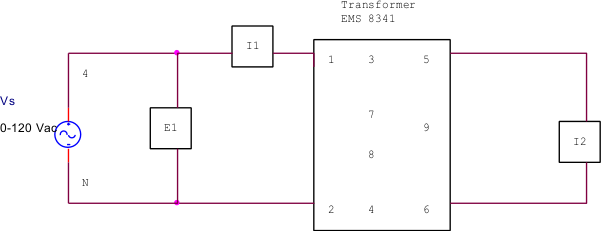
\includegraphics[width=.8\textwidth]{img/circuit_02}
  \caption{Single Phase Transformer Circuit}
  \label{fig:circuit_02}
\end{figure}

\subsection{Saturation}
\begin{figure}[H]
  \centering
  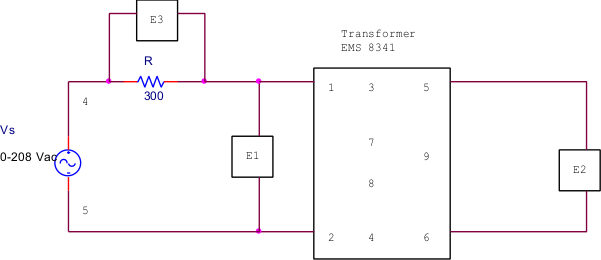
\includegraphics[width=.8\textwidth]{img/circuit_03}
  \caption{Single Phase Transformer Circuit}
  \label{fig:circuit_03}
\end{figure}

\section{Procedure}
\subsection{Voltage Ratios}
\label{part1}
CHANGE ME!! At the EMS workstation, the main power switch of the Power Supply
was verified to be OFF, and the voltage control knob was verified to be
completely counterclockwise. The voltmeter selector switch was set to position
4-N. The RLC circuit shown in Figure~\ref{fig:XXX} was modeled with the
capacitor left out at first. The elements labeled E$_1$ and I$_1$ on
Figure~\ref{fig:XXX} referred to the ammeter and voltmeter Data Acquisition
Interface (DAI) connections. The DAI 24-V supply was connected to the main
Power Supply, and the DAI USB cable was connected to the PC workstation. The
main power switch of the Power Supply was switched to ON.

\subsection{Current Ratio}
\label{part2}
CHANGE ME!! On the PC, the Lab-Volt Data Acquisition Management application was
started, and the file pertaining to the experiment being worked was opened.
Three windows (metering, oscilloscope, and phasor analyzer) were verified to
open up along with the experiment file. The three windows were set to
continuously refresh.

\subsection{Saturation}
\label{part3}
CHANGE ME!! The supply voltage was adjusted to read 24-V. Verification was
obtained by monitoring the EMS analog voltmeter and the digital metering window
on the {PC}.  The load voltage E$_1$, load current I$_1$, the real power
consumed by the circuit, and the phase angle were recorded. In the Phasor
Analyzer window, E$_1$ was selected as the reference phasor. The voltage
control knob was then turn completely counterclockwise and the main power
switch was set to OFF.

CHANGE ME!! The EMS workstation was then reconfigured to include the
capacitance.  The subsequent values included in Table~\ref{tab:XXX} were then
measured.

\section{Results}
\subsection{Voltage Ratios}
\begin{table}[H]
  \centering
  \begin{tabular}{cc}
    \hline
    Winding & Resistance \\
    \# & $\Omega$ \\
    \hline
    1--2 &  7.9 \\
    3--4 & 24.9 \\
    5--6 &  7.9 \\
    7--8 &  9.4 \\
    8--4 & 12.1 \\
    5--9 &  3.6 \\
    9--6 &  4.2 \\
  \end{tabular}
  \caption{Winding Resistances}
  \label{tab:wind_res}
\end{table}

\begin{table}[H]
  \centering
  \begin{tabular}{cccc}
    \hline
    Winding & Primary Voltage & Secondary Voltage & Turn Ratio \\
    \# & E$_1$ V (1--2) & E$_2$ V & N$_\text{P}$:N$_\text{S}$\\
    \hline
    3--4 & 120.3 & 207.2 & 0.58 \\
    5--6 & 119.9 & 119.4 & 1.00 \\
    7--8 & 120.4 &  75.8 & 1.59 \\
    3--7 & 120.3 & 103.6 & 1.16 \\
    8--4 & 120.3 &  27.8 & 4.33 \\
    5--9 & 120.2 &  59.8 & 2.01 \\
    9--6 & 120.1 &  59.7 & 2.01 \\
  \end{tabular}
  \caption{Primary and Secondary Voltages}
  \label{tab:volt_rat}
\end{table}

\subsection{Current Ratio}
\begin{table}[H]
  \centering
  \begin{tabular}{ccc}
    \hline
    E$_1$ & I$_1$ & I$_2$ \\
    V & A & A \\
    \hline
    11.75 & 0.403 & 0.399 \\
  \end{tabular}
  \caption{Winding Resistances}
  \label{tab:curr_rat}
\end{table}

\subsection{Saturation}
\begin{table}[H]
  \centering
  \begin{tabular}{ccc}
    \hline
    Primary Voltage & Secondary Voltage & Exciting Voltage\\
    E$_1$ V (1--2) & E$_2$ V & E$_2$ V\\
    \hline
    10.56 &  10.42 &  2.12 \\
    19.61 &  19.39 &  2.84 \\
    30.90 &  30.60 &  3.57 \\
    40.77 &  40.39 &  4.11 \\
    50.02 &  49.60 &  4.59 \\
    60.76 &  60.27 &  5.12 \\
    70.54 &  70.03 &  5.62 \\
    80.48 &  79.90 &  6.04 \\
    91.36 &  90.73 &  6.59 \\
    99.36 &  98.66 &  7.02 \\
    110.57 & 109.78 &  7.63 \\
    119.85 & 119.07 &  8.20 \\
    130.03 & 129.16 &  8.91 \\
    140.67 & 139.77 &  9.76 \\
    149.73 & 148.70 & 10.70 \\
    160.85 & 159.70 & 12.25 \\
    171.55 & 170.27 & 14.50 \\
    180.38 & 178.92 & 17.11 \\
  \end{tabular}
  \caption{Data for Fig~\ref{fig:circuit_03}}
  \label{tab:circuit_3}
\end{table}

\begin{figure}[H]
  \centering
  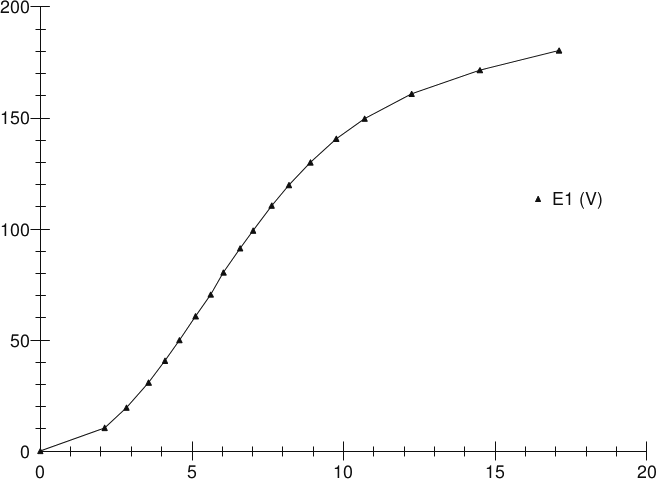
\includegraphics[width=.8\textwidth]{img/graph}
  \caption{Saturation Curve}
  \label{fig:graph}
\end{figure}

\section{Conclusions}
CHANGE ME!!  The effects of different levels of capacitance were observed by
conducting this experiment. The theoretical values for real power, apparent
power, and the phase angle were calculated. Then, the experiment was conducted
to verify the effects of a parallel RLC circuit. These measured results were
differed from the theoretical results because of one underlying reason. The
switch modeling the inductance at the EMS workstation contained an internal
impedance.  This added impedance caused the calculated results to differ from
the measured.  Also, one can see that the voltage measured at E$_1$ fluctuating
throughout the experiment. This fluctuation caused added variations between
measured and theoretical.

\end{document}
